\chapter{Introduction}

Since the invention of smart devices, the mobile traffic has been increasing tremendously over the last decade. According to the recent surveys on mobile traffic by prominent market leaders (Cisco \cite{CISCO14} and Ericsson\cite{Eric15}), the existing mobile traffic is expected to increase $11 \times$ by 2021. The wireless community including the standardization bodies (3GPP) believe that the state-of-the-art standards (fourth-Generation (4G) -- LTE, WiMAX) are not capable of sustaining these demands in the upcoming decade. With this situation in hand, the standardization bodies are currently in the phase of conceptualizing the requirements of the fifth-generation (5G) of mobile wireless systems.
Some of these major requirements are: (i) areal capacity in $\SI{}{bits/sec/m^2}$ must increase by a factor of $1000$ compared to 4G, (ii) low latency of approximately \SI{1}{ms}, and, (iii) energy- and cost-efficient deployment \cite{Qual13, Andrews14}.
 %One of the major goals is to improve the areal capacity ($\SI{}{bits/s/m^2}$) by a factor of 1000 \cite{Qual13, Andrews14}. \tc{To this end, an extension to the already allocated spectrum is of paramount importance.} 
Small cell deployments and an extension to the already allocated spectrum are some of the most promising approaches that allow us to accomplish the aforementioned requirements. These approaches are closely examined in the following paragraphs. 

\subsubsection*{Small Cell}

In the recent past, Small Cells (SCs) have emerged as a potential solution for coverage and capacity enhancements in a network. An SC represents a low power station that ranges from $\SI{10}{m}$ to $\SI{100}{m}$, comparable to the size of a femtocell. The reduced transmit distance accomplished with the deployment of SCs enhances the link quality and aids spatial reuse \cite{Chander08}.
%SC is particularly deployed in a indoor or outdoor environments, these include enterprise, shopping complex or residential \cite{SSF14}. 
As a result, ultra-densification via SCs is envisaged as the absolute paramount for the Fifth-Generation (5G) of wireless systems \cite{Andrews14}.
The capacity, however, increases linearly with the number of SCs, hence, it is infeasible to procure the factor of $1000$ in the areal capacity with ultra-densification alone.
Additionally, backhaul deployment and operation of these substantial number of SCs are cost- and energy-intensive for the mobile operator.




\subsubsection*{Spectrum extension}
Complementing the link quality by means of SCs, the spectrum represents a major contribution to the desired areal capacity. Given the present situation of the spectrum allocated to the mobile applications, it is difficult to procure an extension to already allocated spectrum. Before examining the potential candidates for the spectrum extension, it is necessary to consider the following classification of the spectrum:
%\begin{itemize}
(i) $\ge \SI{6}{GHz}$;
(ii) $\le \SI{6}{GHz}$.
%\end{itemize}
The prime objective of this sort of classification is to shift the focus on the propagation characteristics and the issues thereof.


The spectrum beyond \SI{6}{GHz} largely entails the millimeter Wave (mmW), which is well-known for point-to-point communications. Recently, it is envisaged as a powerful source of spectrum for 5G wireless systems. However, the millimeter wave technology is still in its initial stage and along with complex regulatory requirements in this regime, it has to address several challenges like propagation loss, low efficiency of radio frequency components such as power amplifiers, small size of the antenna and link acquisition \cite{Rapp13}. Therefore, in order to capture a deeper insight of its feasibility in 5G, it is essential to overcome the aforementioned challenges in the near future\nociteK{Kaushik13, Kaushik14_W, Kaushik14_CC, Kaushik14_P, Kaushik15_CC,Kaushik15_ICC, Kaushik15_D, Kaushik16_TWC, Kaushik16_ICC, Kaushik16_CC}.

\tc{Besides the spectrum beyond \SI{6}{GHz}, an efficient utilization of the spectrum below \SI{6}{GHz} presents an alternative solution. The use of the spectrum in this regime (below \SI{6}{GHz}) is fragmented and statically allocated, leading to inefficiencies and the shortage in the availability of the spectrum for new services.} However, it is possible to overcome this scarcity if we manage to utilize this radio spectrum efficiently. In this perspective, \tc{cognitive radio (CR) is foreseen as one of the potential contenders that addresses the spectrum scarcity problem. Since its origin by Mitola \textit{et al.} in 1999, this notion has evolved at a significant pace, and consequently has acquired certain maturity.} However, from a deployment perspective, this technology is still in its preliminary phase. In this view, it is necessary to make substantial efforts that enable the placement of this concept over a hardware platform. This would further facilitate the disposition of CR systems in the upcoming 5G wireless networks. In this regard, this thesis capitalizes on the deployment of the CR system. 

\subsubsection*{Cognitive Radio Systems}
In order to proceed further, it is essential to understand the different CR systems that classified in the literature. An access to the licensed spectrum is an outcome to the paradigm employed by the \tc{secondary user (SU)}. Based on the paradigms described in the literature, all CR systems that provide dynamic access to the spectrum mainly fall under three categories, namely, interweave, underlay and overlay systems \cite{Goldsmith09}. 
\begin{itemize}
\item In Interweave Systems (ISs), the SUs render an interference-free access to the licensed spectrum by exploiting spectral holes in different domains such as time, frequency, space and polarization. 
\item Underlay Systems (US) enable an interference-tolerant access under which the SUs are allowed to use the licensed spectrum (e.g. Ultra Wide Band) as long as they respect the interference constraints of the Primary Receivers (PRs). 
\item Hybrid Systems (HSs) combine the benefits of the IS (agility to detect spectrum holes in different domains) and the US (interference-tolerant capability) to enhance the spectral usage efficiency.  
\item Overlay systems consider the participation of higher layers for enabling the spectral coexistence between two or more wireless networks. 
\end{itemize}
Since the IS, US are HS are closely associated with the physical layer, these systems are mostly considered not only for the theoretical analysis but for practical implementations as-well \citeK{Kaushik13,Kaushik14_CC,Kaushik15_D, Kaushik16_CC}, \cite{Cabric06, Kim10}. Motivated by these facts, this thesis focuses on the performance analysis of these CR systems from a deployment perspective. 


\section{Motivation}
\label{sec:mot}


\subsection{Cognitive Small Cell: A Prominent Use-case}
\begin{figure}[!t]
\centering
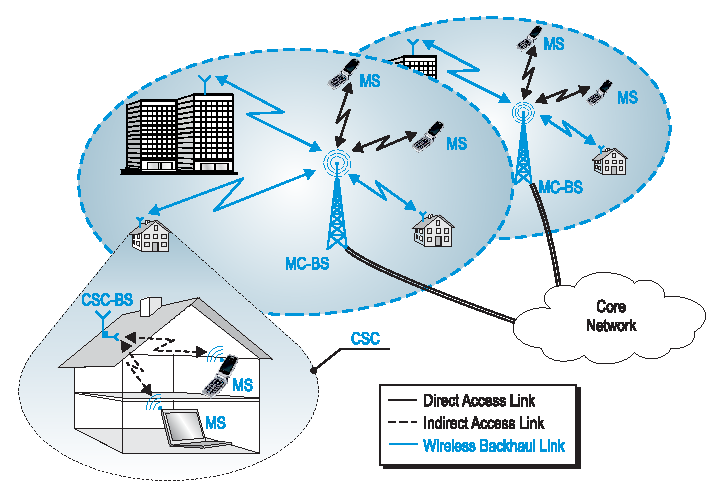
\includegraphics[width = \columnwidth]{figures/Cellular_Scenario_CR6F}
\caption{An illustration of the CSC deployment in a 5G network.}
\label{fig:scenario}
\end{figure}



Following the previous discussion, it is evident that spectrum extension and SCs are key-enablers for the 5G system.
%Recently, ElSawy \textit{et al.} \cite{Elsawy13} have presented Cognitive Small Cell (CSC), a concept that fulfills the capacity demands of the future wireless networks. 
Motivated by this fact, a preliminary concept of Cognitive Small Cell (CSC), a promising approach that jointly enhances the SC deployment and the efficient usage of the spectrum below \SI{6}{GHz}. The notion of CSC has been previously investigated by Elsawy \textit{et al.} \cite{Elsawy13}, where the authors primarily emphasized on the modelling techniques that illustrate the positioning of several CSCs inside the network. In the view of this, the performance analysis of the CSC was constricted mainly to network abstraction. In this article, we provide a deployment-centric viewpoint to ensure a successful integration of CSCs in the 5G network. Consequently, by considering different CR paradigms to enable secondary usage of the licensed spectrum, we illustrate a deeper comprehension of the concept. %, thereby, making it accessible to 5G systems. 
%To strengthen our understanding of CSC, we demonstrate the feasibility of the respective paradigms by means of hardware implementations.
%Pertaining to the deployment, we analyze the true performance of the CSC as a CR application for the mentioned paradigms.  

A comprehensive incorporation of CSC in a preliminary 5G architecture is illustrated in \figurename~\ref{fig:scenario}. From the market analysis, it has been depicted that $70\%$ of the data traffic is originated indoor \cite{Chander08}. In addition, a new range of wireless services, categorized as Internet of Things, will operate from indoor. Thus, the effects will be far more consequential if we consolidate these sources of data traffic by means of SCs deployment. In this regard, it is sensible to consider the residential and enterprise as the main deployment scenarios for the CSC, cf. \figurename~\ref{fig:scenario}. Except for a different coverage regime, the operating principles of these scenarios are analogous.


\section{Main Contributions}

\section{Organization}
